\documentclass[
  bibliography=totoc,     % Literatur im Inhaltsverzeichnis
  captions=tableheading,  % Tabellenüberschriften
 % titlepage=firstiscover, % Titelseite ist Deckblatt
  twocolumn=true, 
]{scrartcl}

\usepackage[T1]{fontenc}
% \usepackage[latin9]{inputenc}
% \setcounter{secnumdepth}{0}
\usepackage{wrapfig}

\addtokomafont{title}{\raggedright}
\addtokomafont{author}{\raggedright}
\addtokomafont{date}{\raggedright}
\addtokomafont{publishers}{\raggedright}


% Paket float verbessern
\usepackage{scrhack}

% Warnung, falls nochmal kompiliert werden muss
\usepackage[aux]{rerunfilecheck}

% unverzichtbare Mathe-Befehle
\usepackage{amsmath}
% viele Mathe-Symbole
\usepackage{amssymb}
% Erweiterungen für amsmath
\usepackage{mathtools}

% Fonteinstellungen
\usepackage{fontspec}
% Latin Modern Fonts werden automatisch geladen
% Alternativ zum Beispiel:
%\setromanfont{Libertinus Serif}
%\setsansfont{Libertinus Sans}
%\setmonofont{Libertinus Mono}

% Wenn man andere Schriftarten gesetzt hat,
% sollte man das Seiten-Layout neu berechnen lassen
\recalctypearea{}

% deutsche Spracheinstellungen
%\usepackage[ngerman]{babel}


\usepackage[
  math-style=ISO,    % ┐
  bold-style=ISO,    % │
  sans-style=italic, % │ ISO-Standard folgen
  nabla=upright,     % │
  partial=upright,   % ┘
  warnings-off={           % ┐
    mathtools-colon,       % │ unnötige Warnungen ausschalten
    mathtools-overbracket, % │
  },                       % ┘
]{unicode-math}

% traditionelle Fonts für Mathematik
\setmathfont{Latin Modern Math}
% Alternativ zum Beispiel:
%\setmathfont{Libertinus Math}

\setmathfont{XITS Math}[range={scr, bfscr}]
\setmathfont{XITS Math}[range={cal, bfcal}, StylisticSet=1]

% Zahlen und Einheiten
\usepackage[
  locale=DE,                   % deutsche Einstellungen
  separate-uncertainty=true,   % immer Unsicherheit mit \pm
  per-mode=symbol-or-fraction, % / in inline math, fraction in display math
]{siunitx}

% chemische Formeln
\usepackage[
  version=4,
  math-greek=default, % ┐ mit unicode-math zusammenarbeiten
  text-greek=default, % ┘
]{mhchem}

% richtige Anführungszeichen
\usepackage[autostyle]{csquotes}
\usepackage{xpatch}

\setkomafont{title}{\normalfont\bfseries}
\makeatletter
\xpatchcmd{\maketitle}{\titlefont\huge}{\titlefont\small}{}{}
\makeatother
% schöne Brüche im Text
\usepackage{xfrac}

% Standardplatzierung für Floats einstellen
\usepackage{float}
\floatplacement{figure}{htbp}
\floatplacement{table}{htbp}

% Floats innerhalb einer Section halten
\usepackage[
  section, % Floats innerhalb der Section halten
  below,   % unterhalb der Section aber auf der selben Seite ist ok
]{placeins}

% Seite drehen für breite Tabellen: landscape Umgebung
\usepackage{pdflscape}

% Captions schöner machen.
\usepackage[
  labelfont=bf,        % Tabelle x: Abbildung y: ist jetzt fett
  font=small,          % Schrift etwas kleiner als Dokument
  width=0.9\textwidth, % maximale Breite einer Caption schmaler
]{caption}
% subfigure, subtable, subref
\usepackage{subcaption}

% Grafiken können eingebunden werden
\usepackage{graphicx}

% schöne Tabellen
\usepackage{booktabs}

% Verbesserungen am Schriftbild
\usepackage{microtype}

% Literaturverzeichnis
\usepackage[
  backend=biber,
]{biblatex}
% Quellendatenbank
\addbibresource{lit.bib}
\addbibresource{programme.bib}

% Hyperlinks im Dokument
\usepackage[
 % german,
  unicode,        % Unicode in PDF-Attributen erlauben
  pdfusetitle,    % Titel, Autoren und Datum als PDF-Attribute
  pdfcreator={},  % ┐ PDF-Attribute säubern
  pdfproducer={}, % ┘
]{hyperref}
% erweiterte Bookmarks im PDF
\usepackage{bookmark}

\usepackage{abstract}

% Trennung von Wörtern mit Strichen
\usepackage[shortcuts]{extdash}

%von Donna LG
\usepackage{graphicx,caption}

\author{\vspace{-3cm}
 % AUTOR A\\%
 Marcel Karas
  \(\href{mailto:marcel.karas@studio.unibo.it}{marcel.karas@studio.unibo.it} \)
  % \and%
  % AUTOR B\\%
  % \href{mailto:authorB@udo.edu}{authorB@udo.edu}%
}
\publishers{Universita di Bologna – Faculty of Physics}


\begin{document}

\title{\mytitle}

\author{Marcel Karas}
\email[]{marcel.karas@studio.unibo.it}
\affiliation{Department of Physics, Universita di Bologna}
%\affiliation{Universita di Bologna}

\date{\today}

%Objectives (scope of the investigtion)
%reference to materials and methods
%summary of results and conclusions
%Hypothesis

Quantum dots made out of semiconductor materials have tuneable optical properties defined by quantum confinement and material mixture. 
Here, the concentration of Selenium and Sulfur in a quantum confined material can be determined by a photoluminescence measurement.
% background
% brief review of previous research (cite)
% reson why the research was undertaken
% Hypothesis
% explenation of techniques and why they ve been chosen
% objectives = what you hope to achieve
% brief reference to the main outcome
\section{Introduction}
\label{sec:Introduction}

Luminescence is a phenomenon where a sample of any kind get energetically excited and thus emits light of a material and structural specific spectrum.
But also, it is used in nowadays consumer technologies like TV screens. 
In this case, photoluminescence is used to characterize the specifications of three samples, which are semiconductor compounds of the same elements but in different concentrations.
In the following, the samples, as well as the process of photoluminescense, are recalled.

\subsection{Photoluminescense in Semiconductors}
\label{sec:PLS}

Semiconductors are characterized by a bandgap of $\SI{2}{\eV}$ to $\SI{4}{\eV}$, an almost completely filled valence band and an almost completally empty conductance band \cite[391]{festkorperphysik}.
Here, a lightsourse like a LED or Laser is able to excite some electrons from the valence band up into the conductance band, as long as the photoenergy is bigger then the bandgap of the sample.
The electrons loose energy by exciting lattice vibrations, and by reaching the minimum of the conductance band, they may recombine with a hole in the valence band, emmitting a photon with the energy of the band gap.
Here, the equation
\begin{equation}
    h\nu = E_{\text{g}}
\end{equation}\label{eq:h}
holds, where $\nu$ is the photons frequency, and $E_\text{g}$ the band gap.
One easily can see, that the expected frequency of the emitted photons is smaller than the frequency of the pump. 
Nevertheless, due to thermal affects a thermal spread along the energy of the bandgap, and thus a widening of the spectrum around a $\lambda_\text{peak}$ is expected.
Using a spectrometer, this wavelengh can be found, and used to estimate the bandgap energy
\begin{equation}
    E_{\text{g}} = \frac{h\c}{\lambda_\text{peak}}.
\end{equation}

\subsection{Samples}
\label{sec:samples}

There are three $\ce{CdS_x Se_{1-x}/ZnS}$ samples to analyze, where all of them can be described as quantum dots, as the $\ce{ZnS}$ has a bigger bandgap than the $\ce{CdS_xSe_{1-x}}$ molecule, 
thus it acts as a potential barrier.
This provides a confinement potential. The impact of quantum dots on the spectrum is referred in chapter \ref{sec:QD}.
The molecules of $\ce{CdS_x Se_{1-x}/ZnS}$ with a unknown concentration $x$ are submerged in tulene.
The relation between the concentration $x$ and the material's bandgap is mentioned in chapter \ref{sec:SemAll}.

Another sample is methylammonium lead bromide ($\ce{MAPbBr_3}$), a hybrid perovskite single crystal, which is a material used in new approaches of optoelectronic devices.

\subsection{Semiconductor alloys}
\label{sec:SemAll}

Under preserving the lattice structure of the crystal but subseducing one compuond of a semiconductor alloy, the bandgap and the lattice constant changes.
The dependency can be non-lineary, thus a bowing parameter $b$ is introduced. 
The dependency of the bandgap from the subsedution of $\ce{S}$ with $\ce{Se}$ in an alloy with $\ce{Cd}$, quantified by the mentioned concentration (of $\ce{S}$) is given by
\begin{align*}
    E_g(\ce{Cd S_x Se_{1-x}}) &= x \times E_g(\ce{Cd S}) + (1-x) \\ &\times E_g(\ce{Cd Se}) - bx(1-x).
\end{align*}

\subsection{Quantum dot spectra}
\label{sec:QD}

A quantum dot is a one-dimensional potential well, in which the solution of the Schrödinger equation for the electrons gives a discrete energy spectrum, comparable to the one of a single atom.
The lowest available energy state depends on the size of the smallest dimension which here is given by the molecule size.
In the undertaken photoluminescence measurement the emission primarily comes from a relaxation of the lowest energy electron in the conductance band to the highest energy state of the valence band, as explained in chapter \ref{sec:PLS}.
Thus, the dimension of the quantum dot, determining the lowest energy state, is the parameter to set, in order to get the samples $\ce{S}$ concentation out of the spectral information.

\begin{figure*}
  \centering
  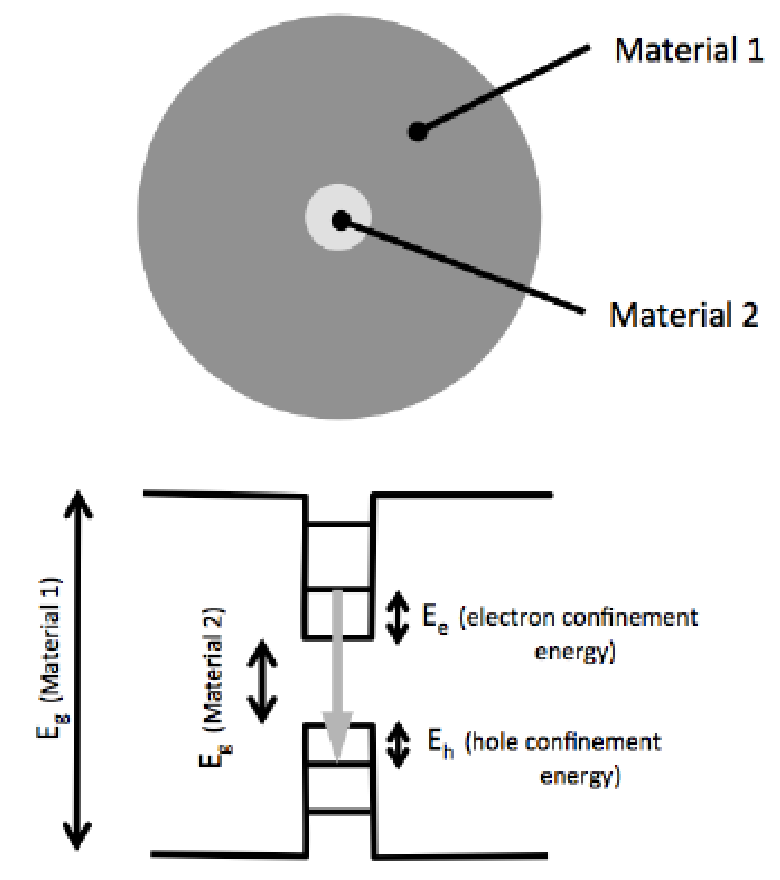
\includegraphics[width=0.35\textwidth]{graphics/QD.png}
  \caption[width=0.4\textwidth]{Structure of a spherical quantum dot and the potential well, created by the surrounding of a material with a bigger bandgap. The optical excitation energy depends not only on the samples band gap $E_g$, but also on the confinement energies due to the quantum dot dimensions\cite{instruction}.}
  \label{fig:QD}
\end{figure*}

As seen in figure \ref{fig:QD}, the optical transition energy is given by
\begin{equation}
    h \nu = E_g + E_e + E_h,
\end{equation}
where $E_g$ is the fundamental bandgap of the material and $E_{e/h}$, the confinement energy for electrons/holes.
Assuming a symetrical quantum dot with a radius $r$, and a linearly on the composition dependent effective mass of the electrons and holes
\begin{align*}
m_e^*(\ce{Cd S_x Se_{1-x}}) &= x m_e^*(\ce{Cd S}) \\ &+ (1-x)m_e^* (\ce{CdSe}) \\
m_h^*(\ce{Cd S_x Se_{1-x}}) &= x m_h^*(\ce{Cd S}) \\ &+ (1-x)m_h^* (\ce{CdSe}),
\end{align*}
for the first confined state one gets
\begin{equation}
    h \nu = E_g + \frac{h^^2}{8er^^2}(\frac{1}{m_e^*} + \frac{1}{m_h^*}).
\end{equation}\label{eq:QD}

\subsection{Experimental setup}
\label{sec:setup}

As lightscources there are used a UV 395 LED as well as a 375nm LDH laser Diode.
The Thorlabs CCS200 Spectrometer is connected with a fiber optic which can be positioned next to the sample. 
In order to minimalize the noise of the exciting light source, a perpendicular positioning to it is used.
The Spectrometer uses a grating in order to project one wavelength onto a CCD linear image sensor.
The wavelength intensity scan can be acquired by moving a mirror. This happens automatically, such that a wavelength-intensity plot is available in the acquisition software.

As there is expected to have noise from external light sources during the experiment, a background measurement for the LED setup is needed.
This can be substracted from the signal later on.
For the laser setup, a darkening curtain is used. 
To overcome statistical fluctuations, the integration time of the acquisition is set to the highest possible level without saturation occurring.

%pictures and spectra
%tables and graphs
%statements of the result

%%% three subfigures next to each others
% \begin{figure*}
%     \centering
% \begin{subfigure}{.3\textwidth}
%     \centering
%     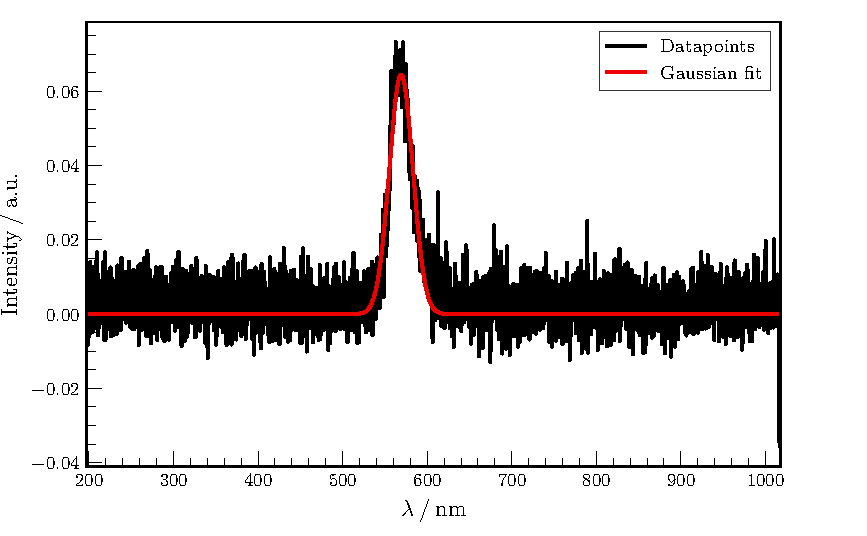
\includegraphics[width=\textwidth]{plots/LED-Green.pdf}
%     \caption{Green LED lightsourse}
%     \label{fig:LEDG}
% \end{subfigure}
% \begin{subfigure}{.3\textwidth}
%     \centering
%     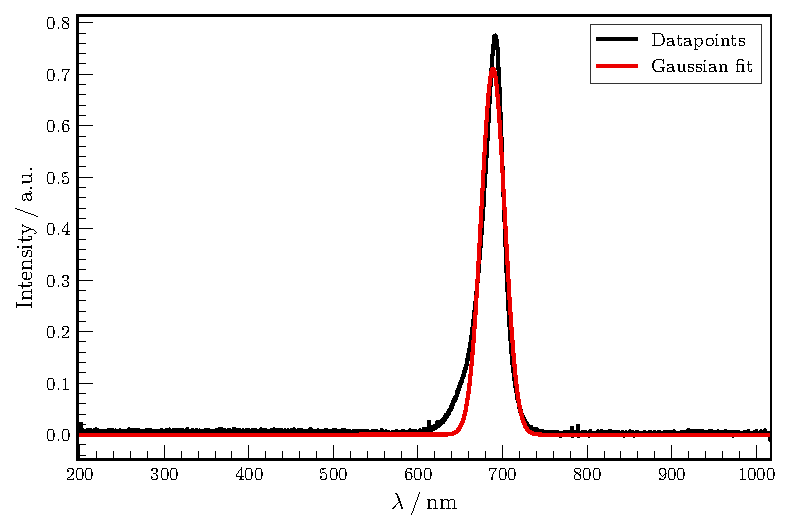
\includegraphics[width=\textwidth]{plots/LED-Red.pdf}
%     \caption{Red LED lightsourse}
%     \label{fig:LEDR}
% \end{subfigure}
% \begin{subfigure}{.3\textwidth}
%     \centering
%     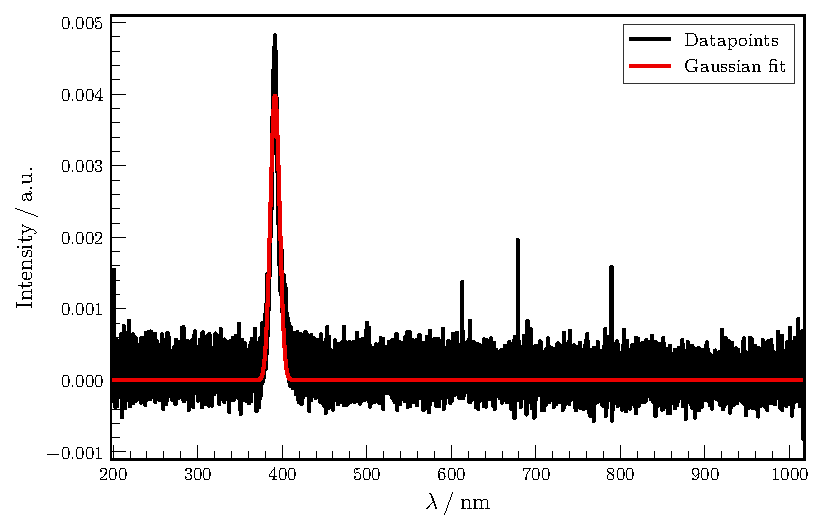
\includegraphics[width=\textwidth]{plots/LED-UV.pdf}
%   \caption{UV LED lightsourse}
%     \label{fig:LEDUV}
% \end{subfigure}
% \caption{Spectral measurement of different LED lightsourse. A Gaussian fit is implemented around the emmision peak.}
% \end{figure*}

%%one figure inside the collums
% \begin{figure}
%     \captionsetup{width=0.9\linewidth}
%     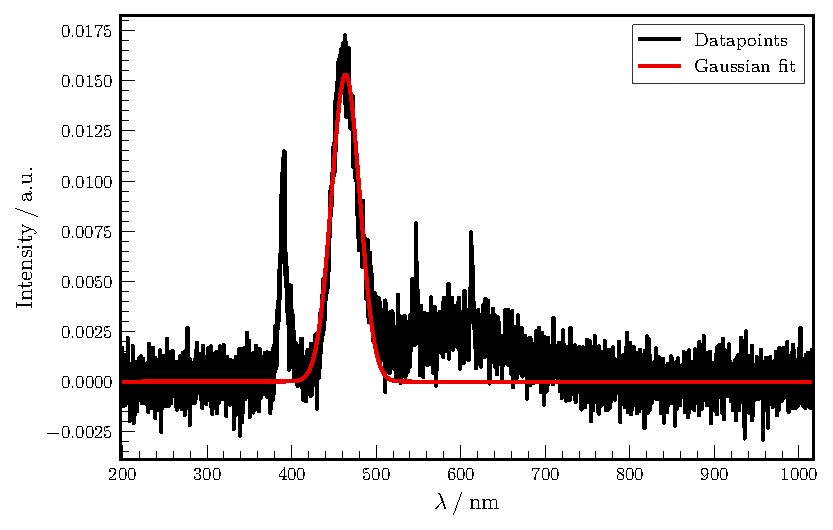
\includegraphics[width=0.5\textwidth]{plots/Samp_A_D.pdf}
%   \caption{Spectral measurement of sample A, excited by a UV-LED lightsource. A Gaussian fit of the peak contributed by luminescense is implemented.}
%     \label{fig:Samp_A_D}
% \end{figure}

\section{Results}
\label{sec:Results}

All characterization steps are done for both samples, where sample A is produced by a perovskite deposited with a slowly evaporated dissolvant 
and sample B with a fast crystallization of the active perovskite layer by introducing an antisolvant.

\subsection{Optic analyzis}
\label{sec:optic-analyzis}

\begin{figure*}
    \centering
\begin{subfigure}{.4\textwidth}
    \centering
    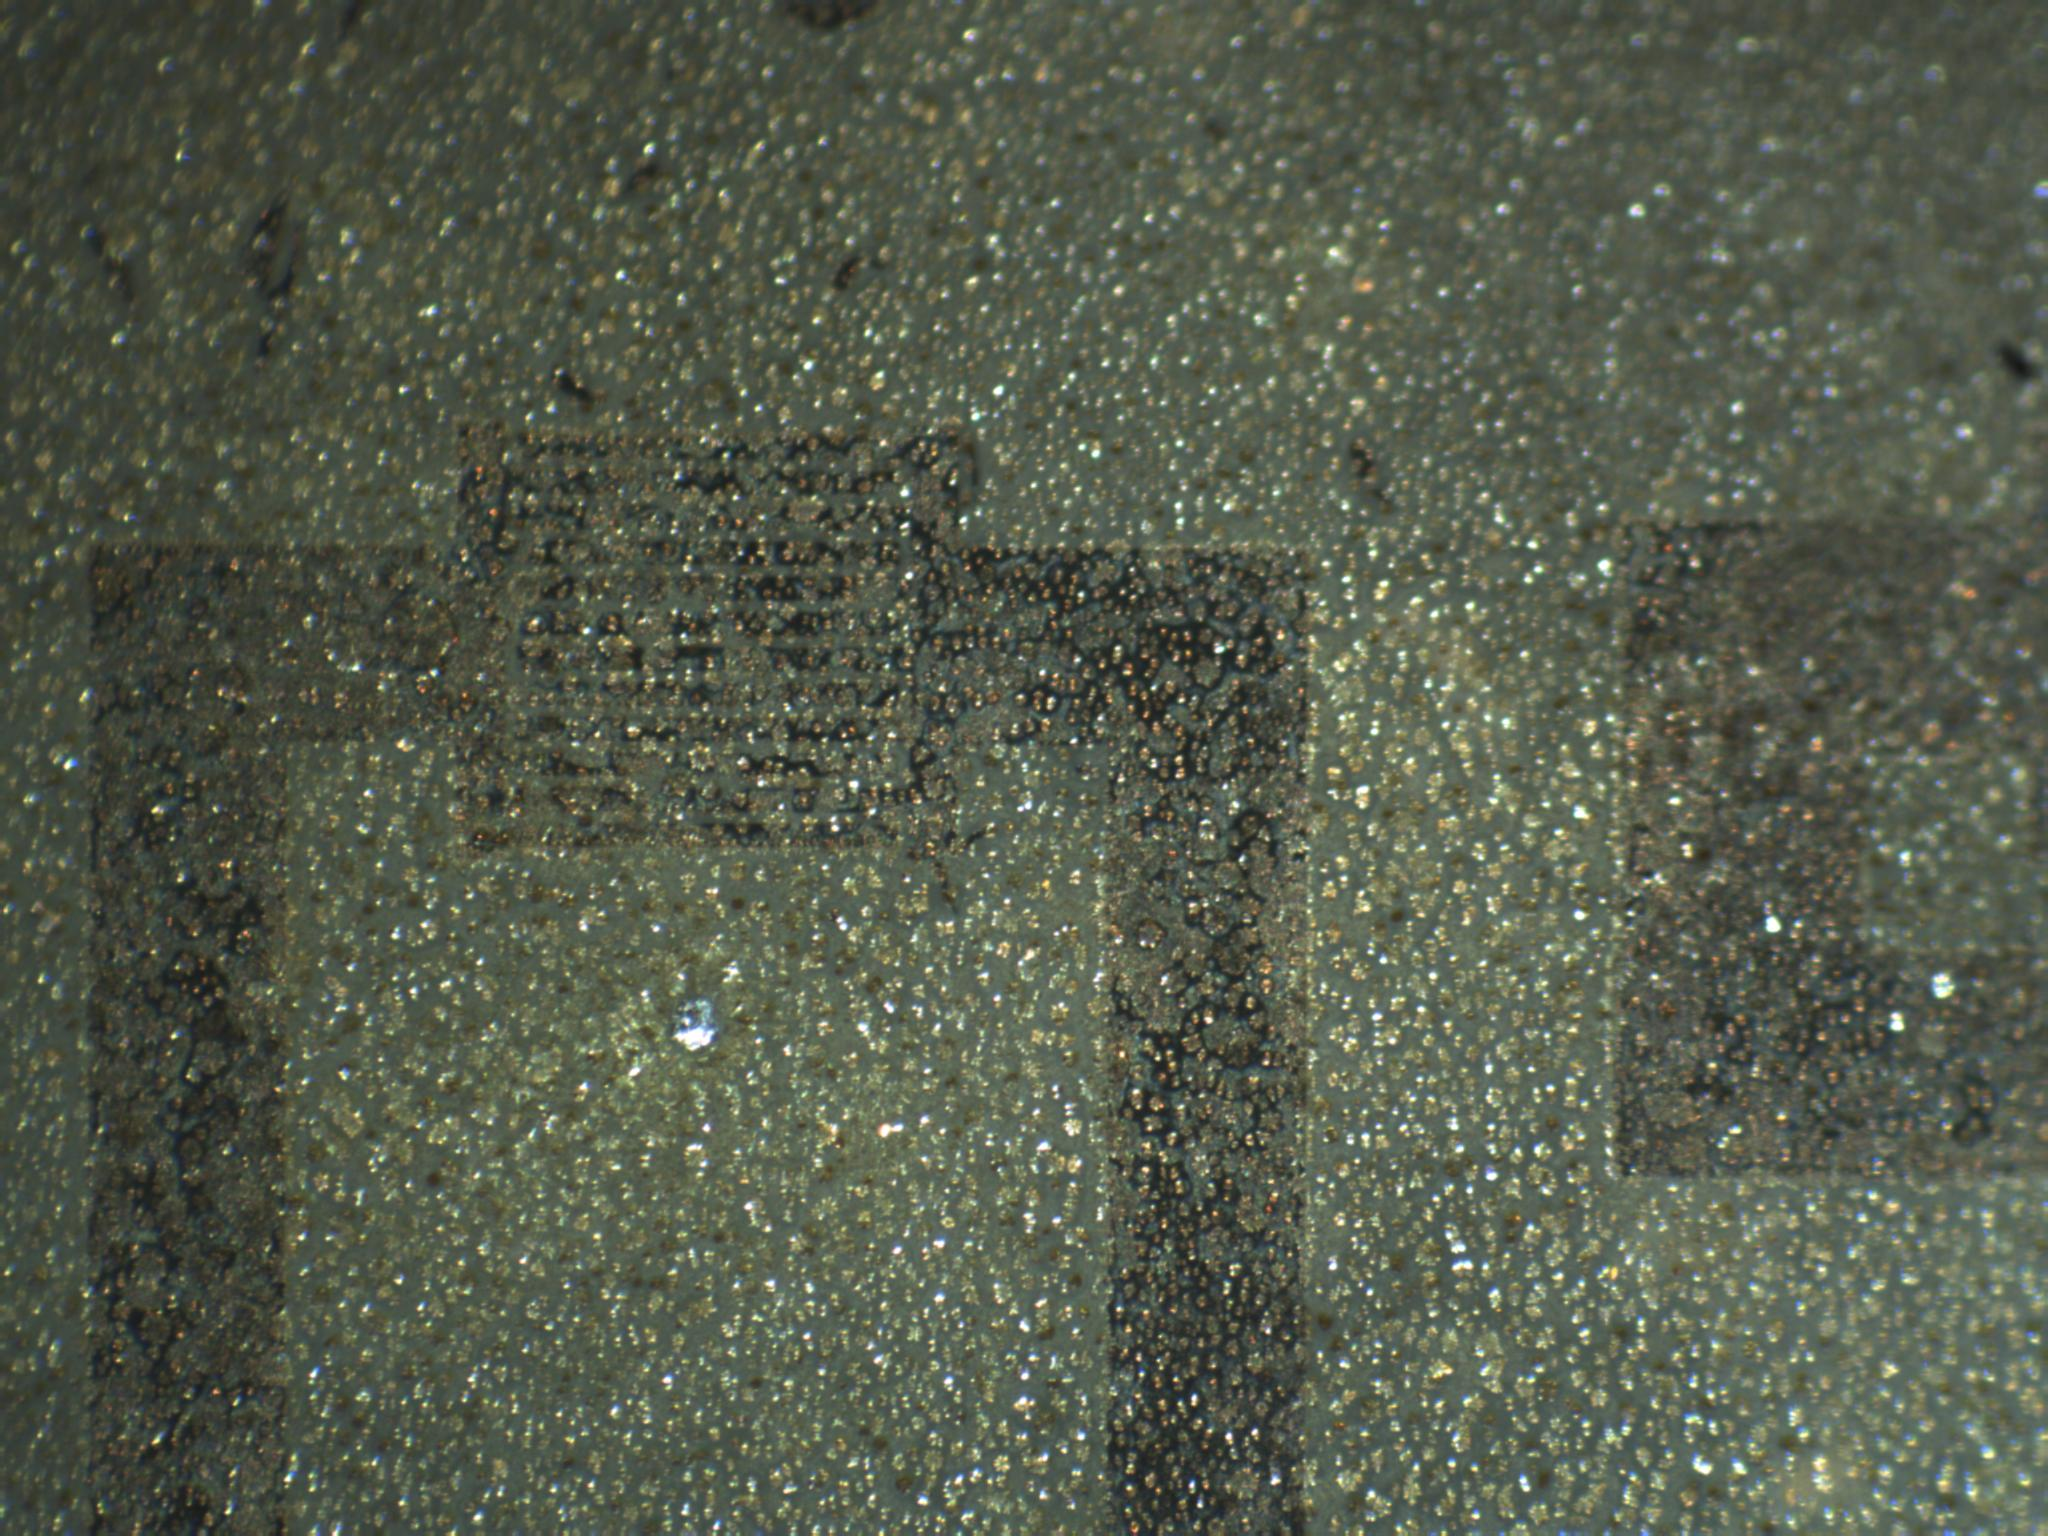
\includegraphics[width=\textwidth]{Data/SampleA_2xzoom.jpg}
    \caption{Front lightning}
\end{subfigure}
\begin{subfigure}{.4\textwidth}
    \centering
    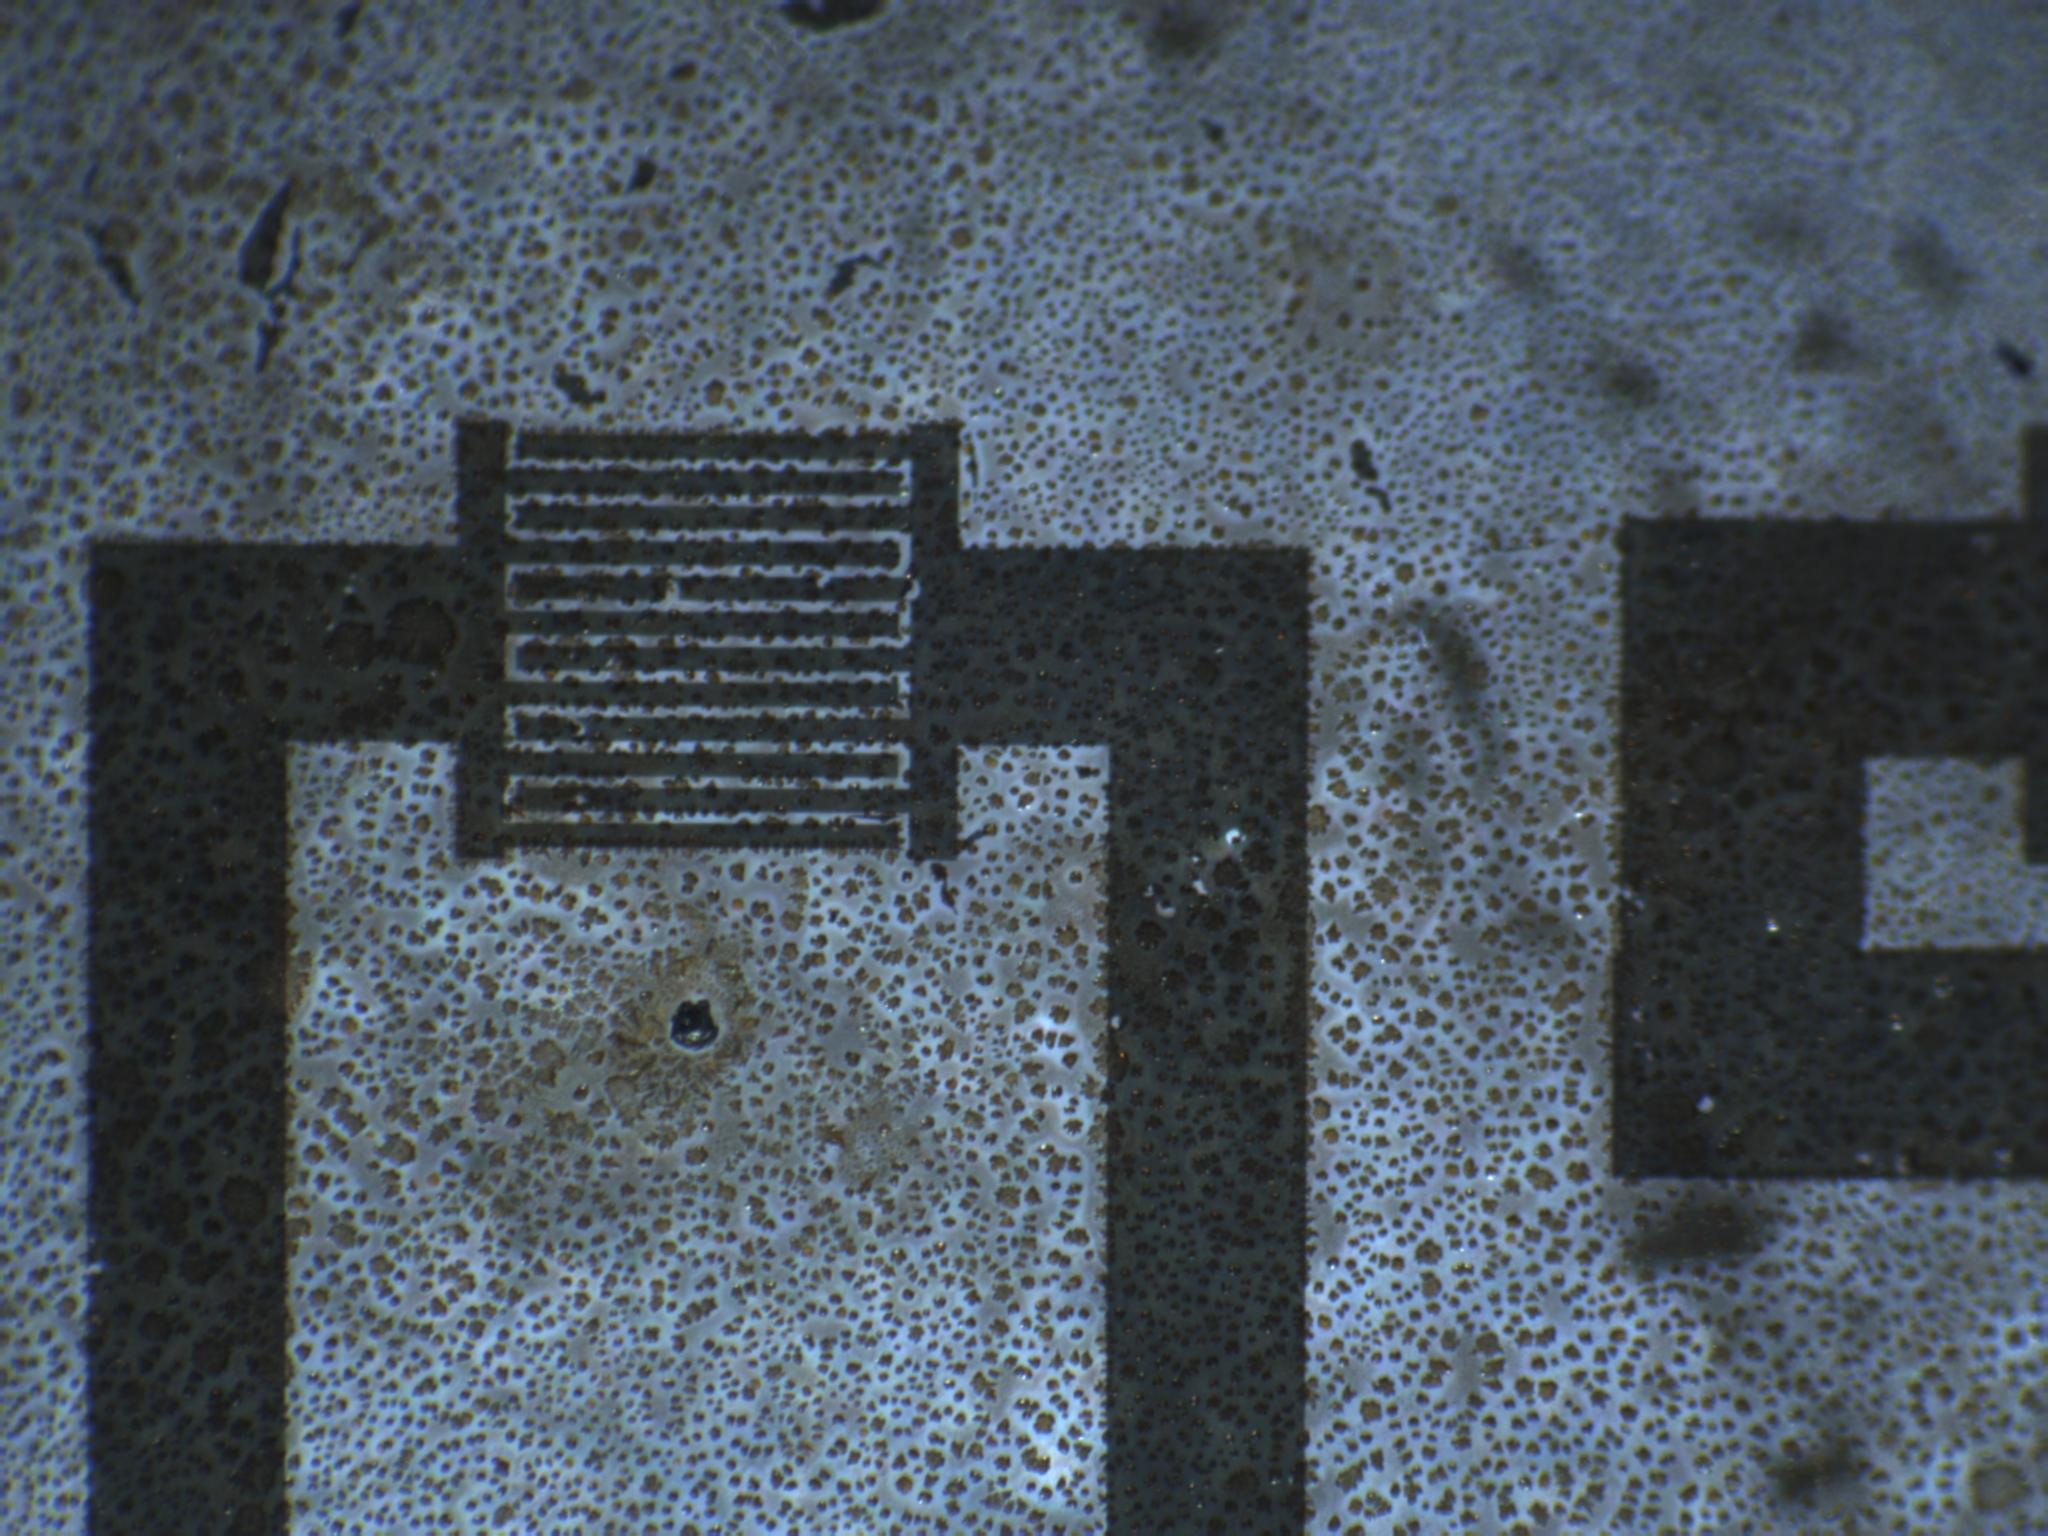
\includegraphics[width=\textwidth]{Data/SampleA_x2zoom_transmission.jpg}
    \caption{Background transmission lightning}
\end{subfigure}
\caption{Microscopic photography with x2 zoom, of no-antisolvant sample A.}\label{fig:optic-A}
\end{figure*}


\begin{figure*}
    \centering
\begin{subfigure}{.4\textwidth}
    \centering
    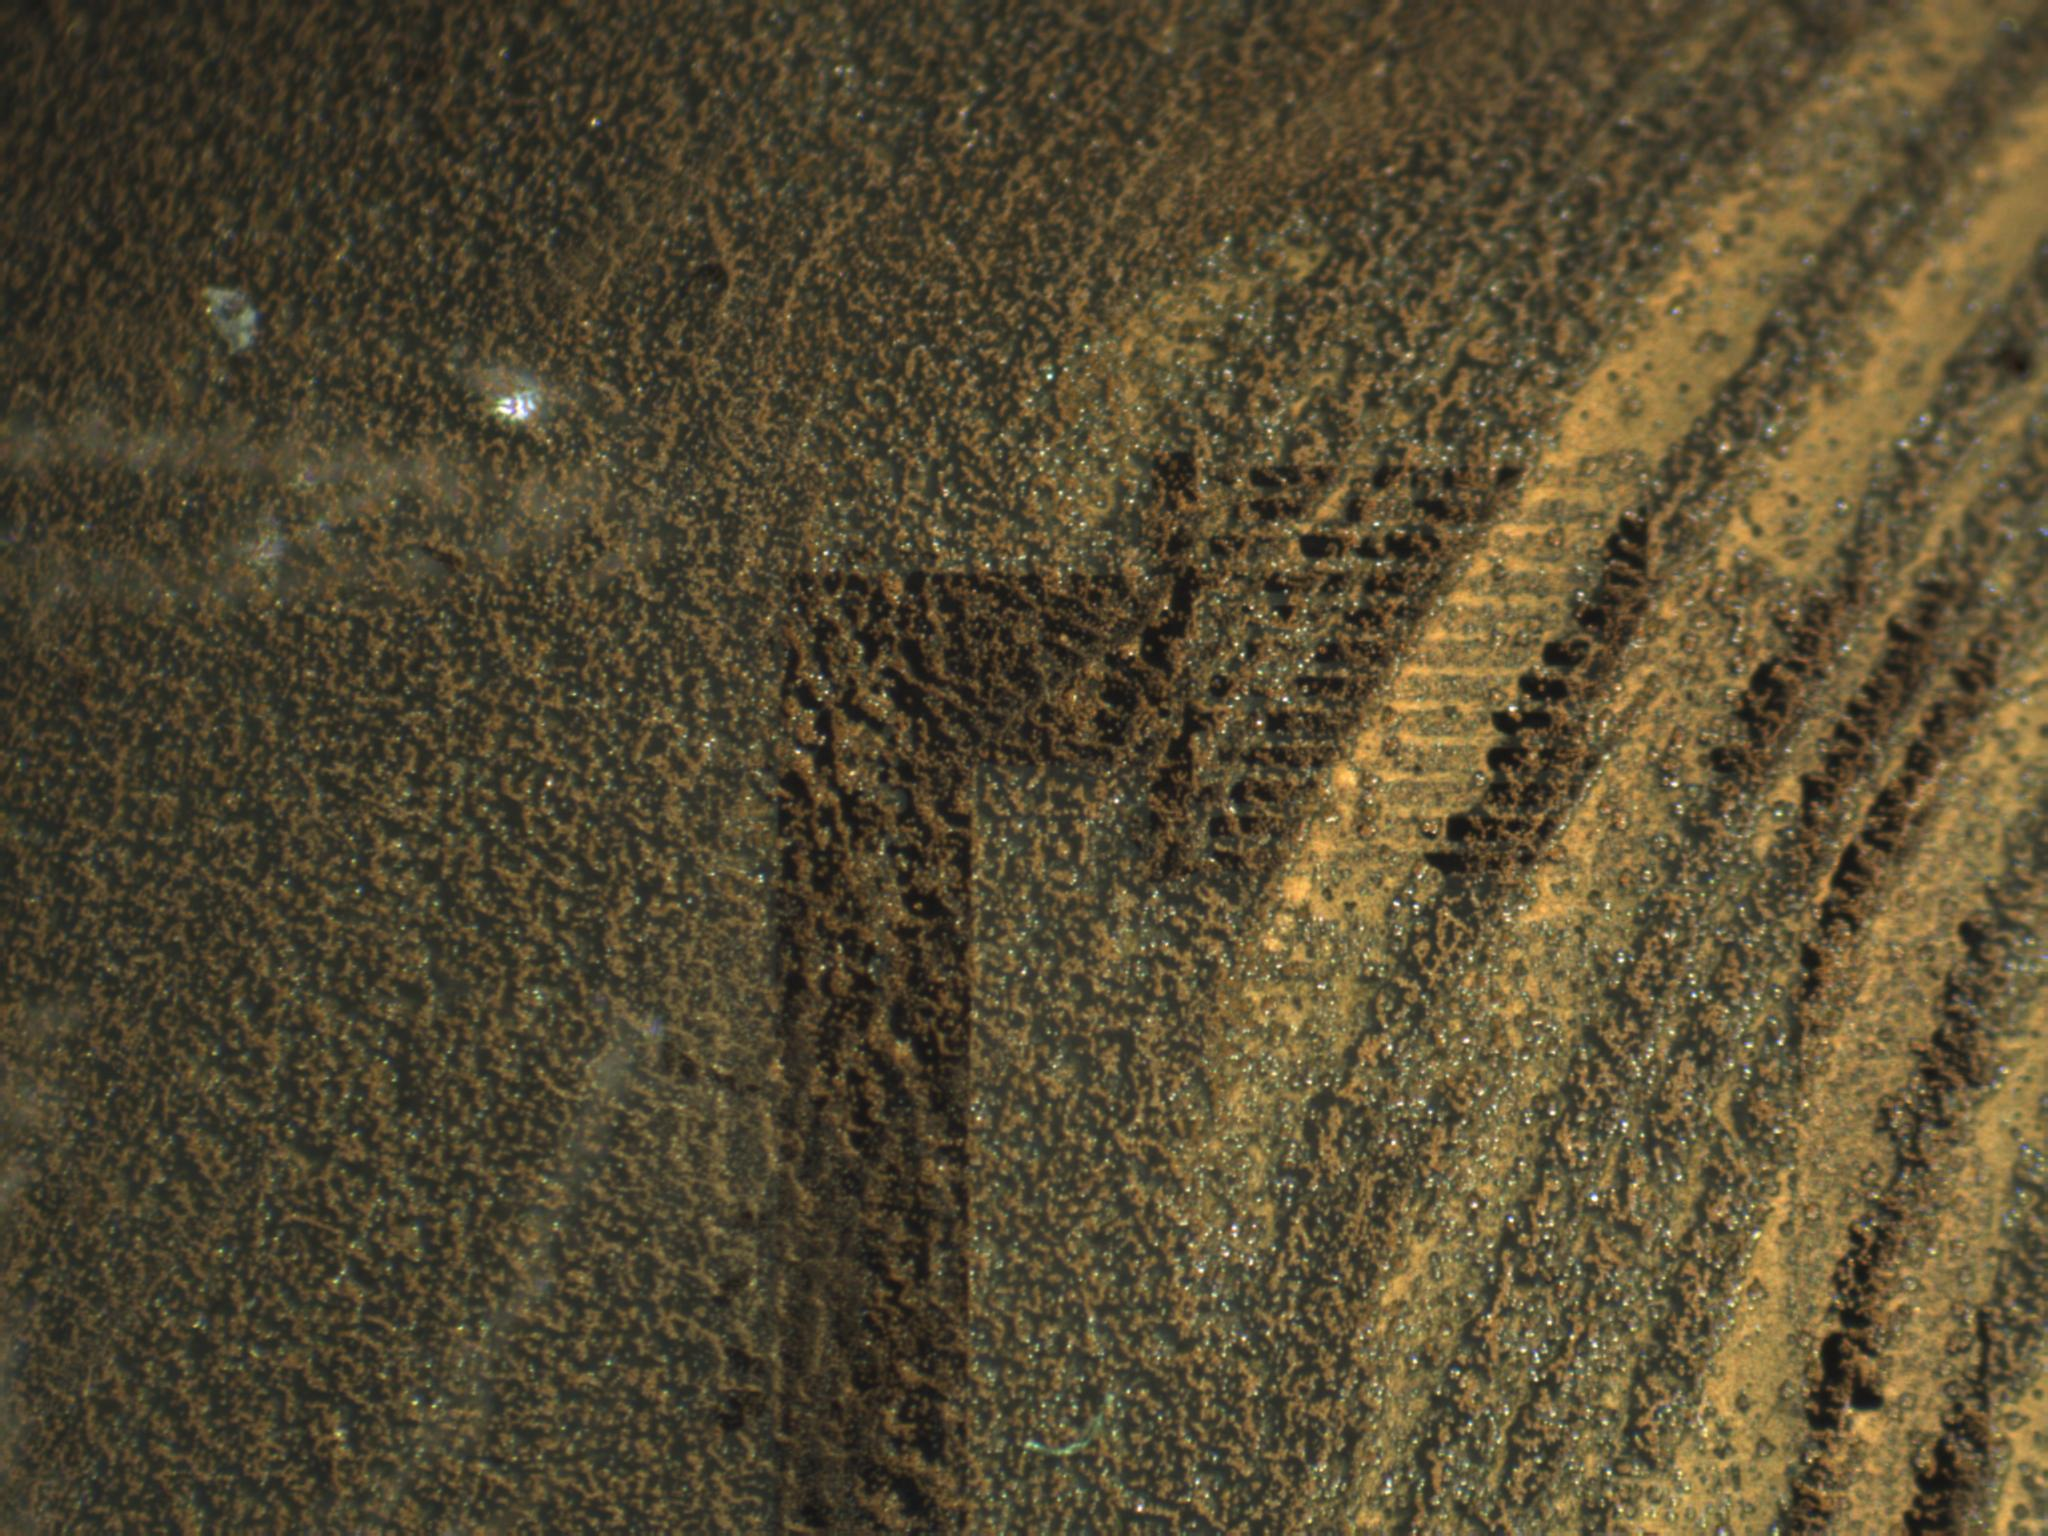
\includegraphics[width=\textwidth]{Data/SampleB_2xzoom.jpg}
    \caption{Front lightning}
\end{subfigure}
\begin{subfigure}{.4\textwidth}
    \centering
    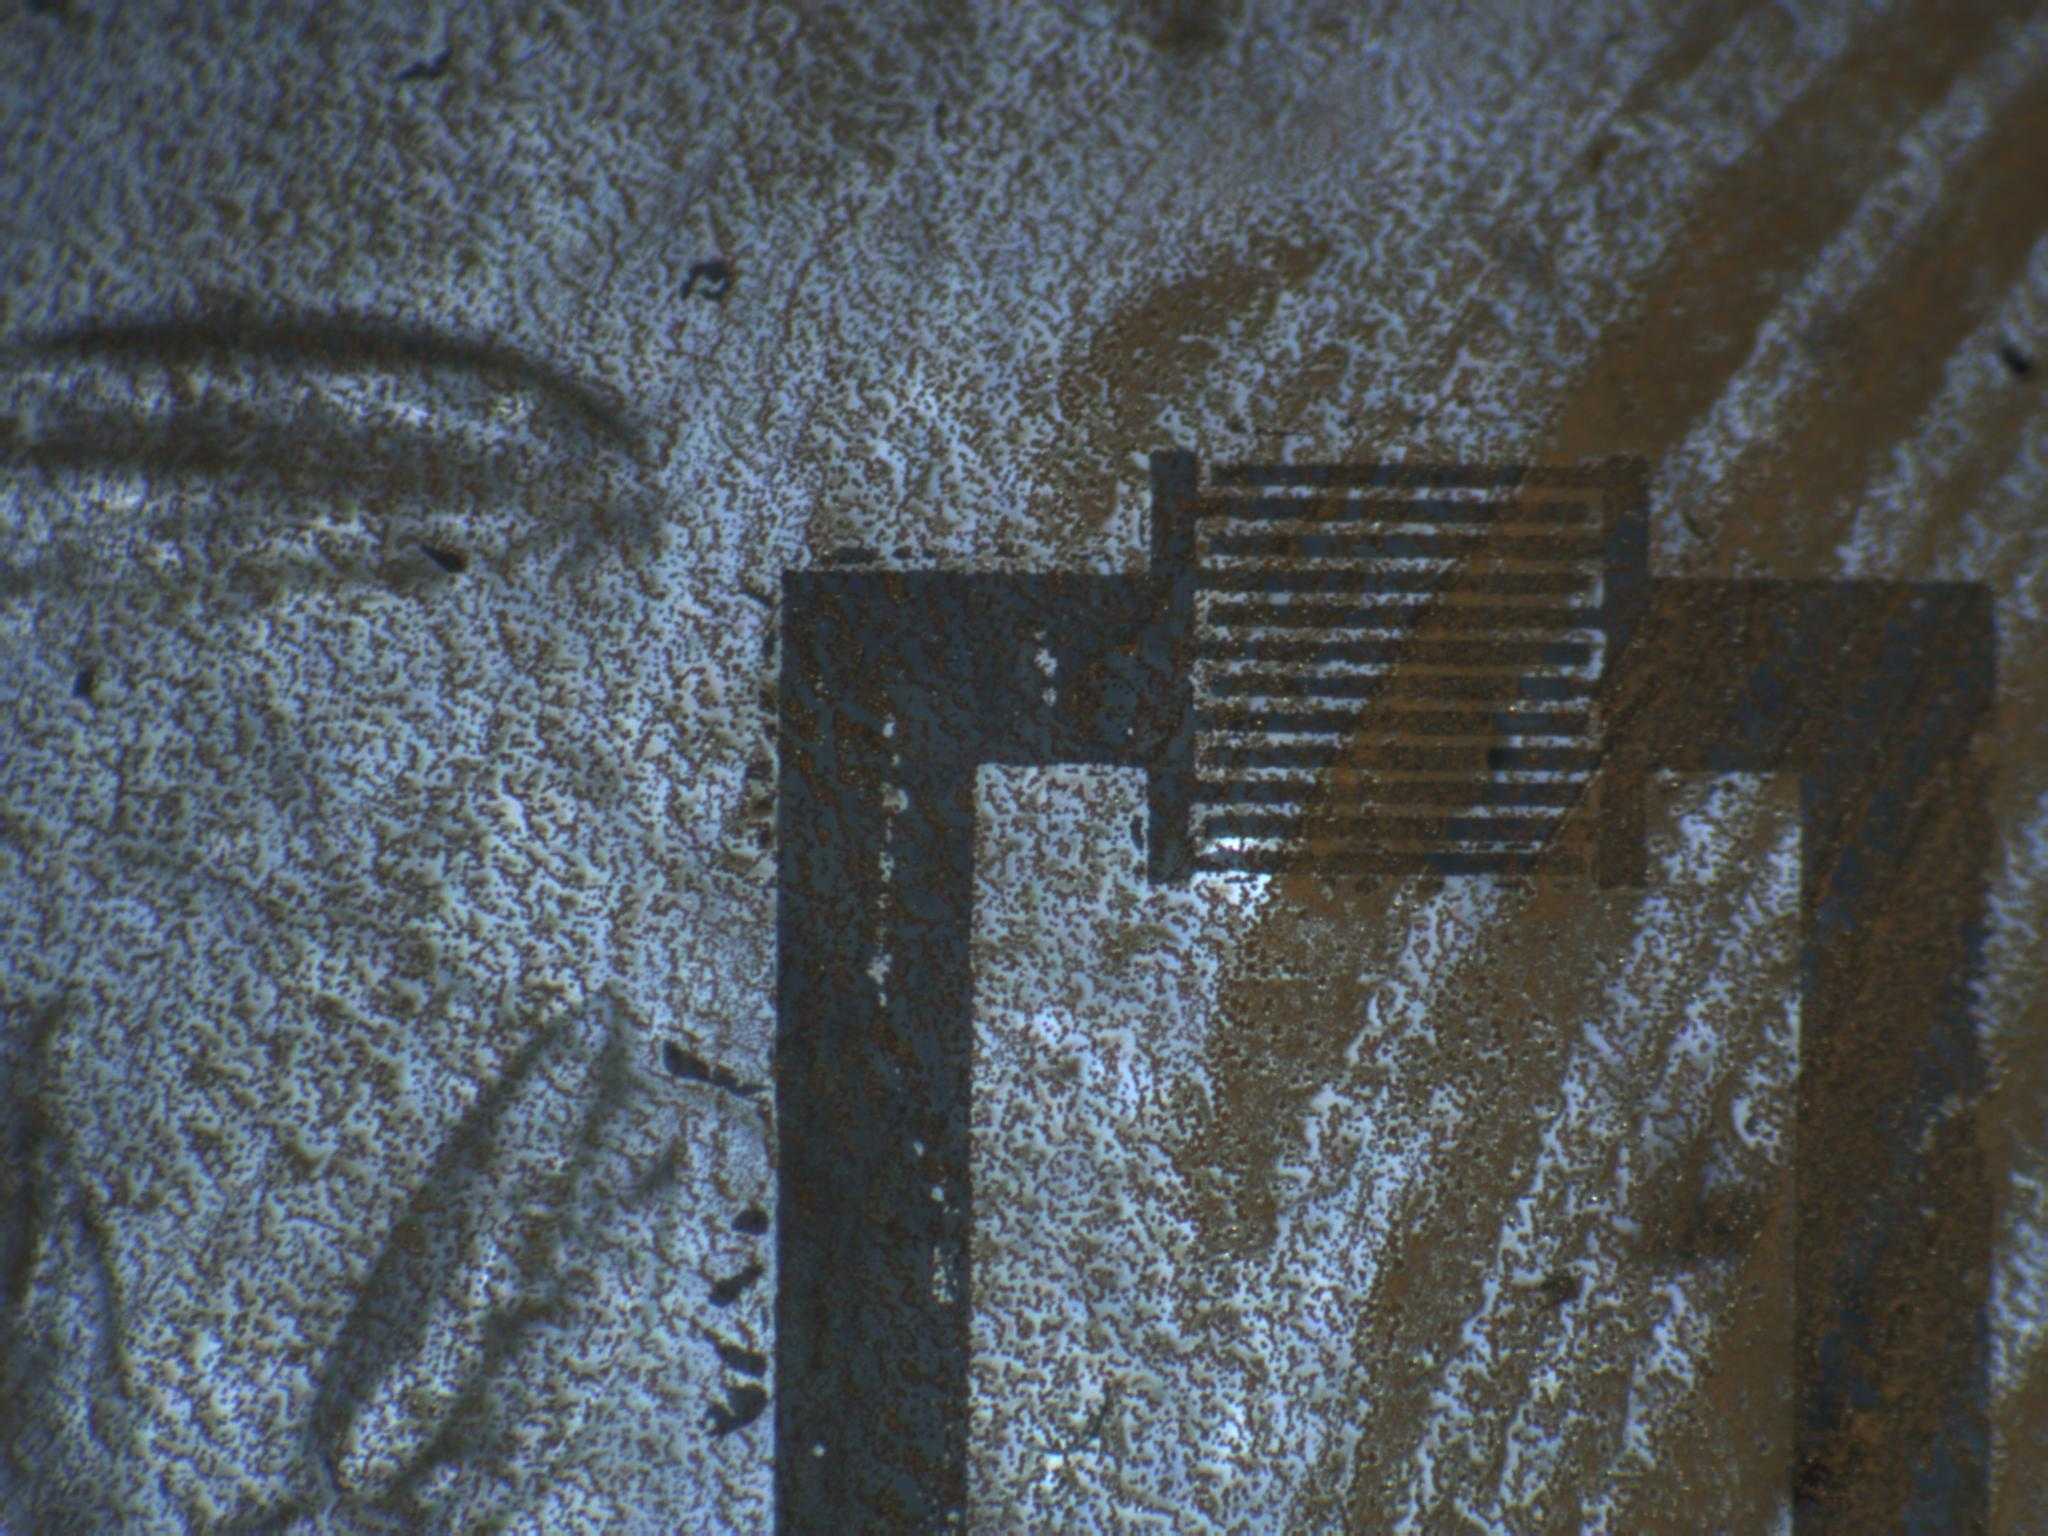
\includegraphics[width=\textwidth]{Data/SampleB_x2zoom_transmission.jpg}
    \caption{Background transmission lightning}
\end{subfigure}
\caption{Microscopic photography with x2 zoom, of antisolvant sample B.}\label{fig:optic-B}
\end{figure*}

In all pictures the contacts seem to be well shaped, so one can expect a functioning electronic connection.
Comparing the figures \ref{fig:optic-A} and \ref{fig:optic-B}, one can see that the reflecting crystals on the surface appear much smaller, almost like a kind of mud on the sample B.
Also the color intensity is stronger for sample B.

\subsection{Electronic analyzis}
\label{sec:elec-analyzis}

\begin{figure*}
    \centering
\begin{subfigure}{.4\textwidth}
    \centering
    \includegraphics[width=\textwidth]{plots/A_dark.pdf}
    \caption{dark}
\end{subfigure}
\begin{subfigure}{.4\textwidth}
    \centering
    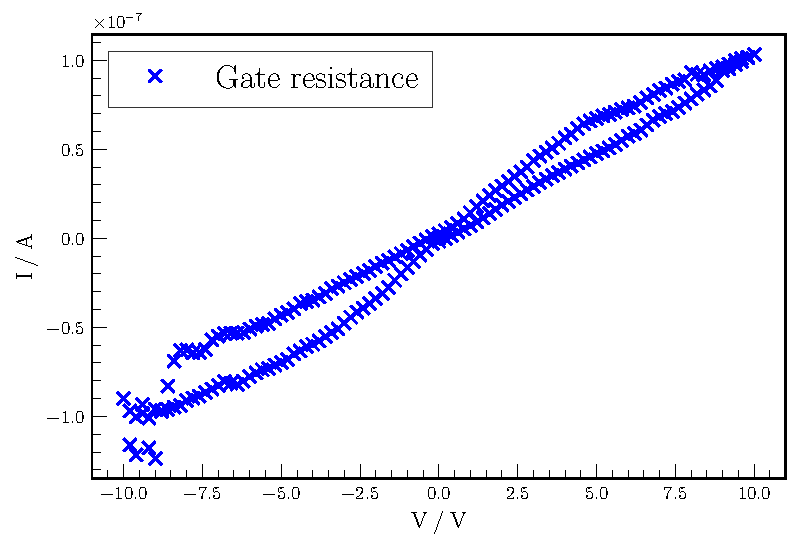
\includegraphics[width=\textwidth]{plots/A_light.pdf}
    \caption{illuminated}
\end{subfigure}
\caption{Gate hysterisis in a V-I plot of the sample A in dark and luminated conditions.}\label{fig:hyst-A}
\end{figure*}


\begin{figure*}
    \centering
\begin{subfigure}{.4\textwidth}
    \centering
    \includegraphics[width=\textwidth]{plots/B_dark.pdf}
    \caption{dark}
\end{subfigure}
\begin{subfigure}{.4\textwidth}
    \centering
    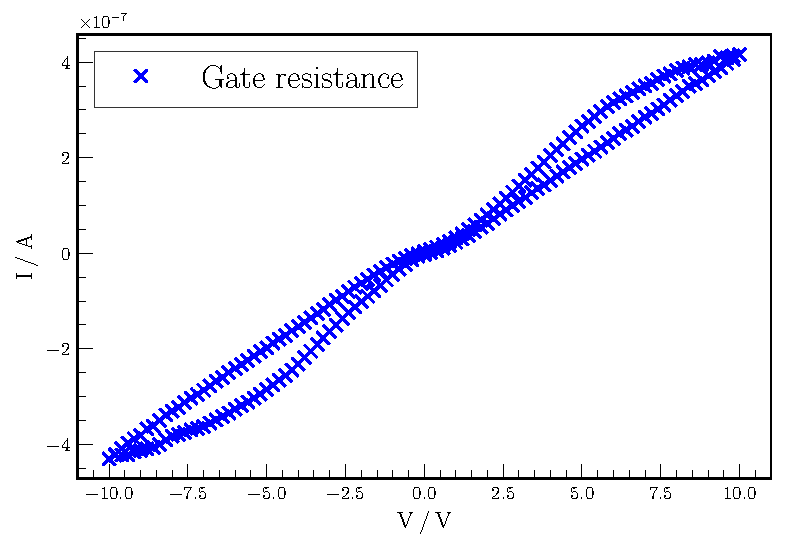
\includegraphics[width=\textwidth]{plots/B_light.pdf}
    \caption{illuminated}
\end{subfigure}
\caption{Gate hysterisis in a V-I plot of the sample B in dark and luminated conditions.}\label{fig:hyst-B}
\end{figure*}

For both samples, one can see a hysteresis of the gate circuit in figure \ref{fig:hyst-A} and \ref{fig:hyst-B}.
Further, the slope which is proportional to the conductivity increases, when the sample is luminated. 
In other words, the resistance of the sample decreases as the sample is illuminated, so both of the samples are sufficient to be used as a linear photodetector, combined with a resistivity measurement aparatus.
 
Refering figure \ref{fig:dynamic}, which shows the time dependent gate current while the light exposion is changed from dark to bright every 5 seconds, shows clearly a current change.
Therefore, it is shown, that the sample circuit can be used as a on/off photodetector.

\begin{figure}
    \captionsetup{width=0.9\linewidth}
    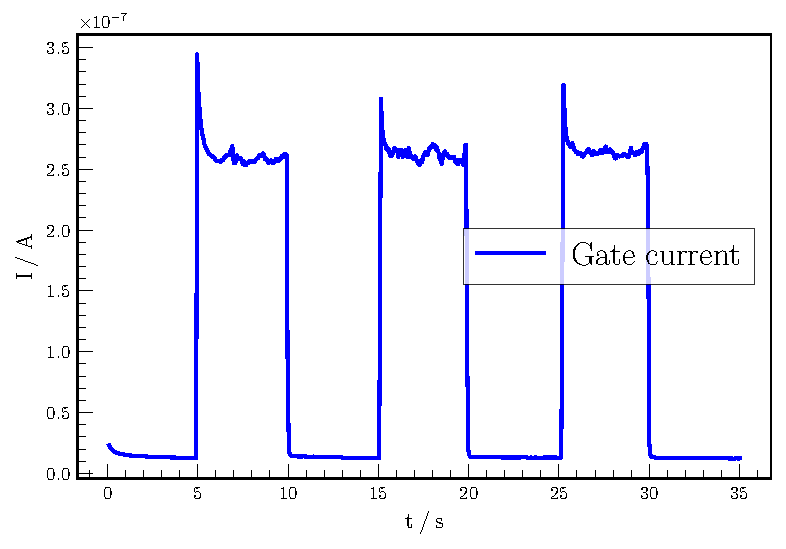
\includegraphics[width=0.5\textwidth]{plots/dynamic.pdf}
  \caption{Gate current of sample B, whiile the illumination is turned on and off every $\SI{5}{\s}$.}
    \label{fig:dynamic}
\end{figure}

% luminated = steigung I/U größer = conductance größer = widerstand kleiner
%interpretation
%comparing and contrasting to litearture
%explain errant data, find possible error sources
%What do the results mean?
%(May it be added in the results"?)
\section{Discussion}
\label{sec:Discussion}

%reaching back to introduction
%suggest improvements
%(highlight importance of results)
\section{Conclusion}
\label{sec:Conclusion}



%\section{\label{sec:References}References}
%\noindent Referencing should be done using BibTeX.
%\section{\label{sec:Conclusion}Final Checklist}

%\begin{itemize}[label=$\Box$]
%\item Think critically about all of your own claims {\em and} about all of the claims made by your coauthors. If you do not understand something that your coauthor has written in the draft, push back until you do understand, then suggest an alternative phrasing to clarify the manuscript or figure.
%\end{itemize}

%\begin{acknowledgments}
%We acknowledge advice from Jessie Zhang and Harry Pirie to produce Fig.\ \ref{fig:pixels}.
%\end{acknowledgments}

%\appendix


\printbibliography{}

\end{document}
